\documentclass[
  bibliography=totoc,     % Literatur im Inhaltsverzeichnis
  captions=tableheading,  % Tabellenüberschriften
  titlepage=firstiscover, % Titelseite ist Deckblatt
  parskip=half, % !!! halbzeiliger vertikaler Abstand (siehe Latex-Skript S.125)
]{scrartcl}

% !!! Python in Latex
\usepackage{pythontex}

% !!! zum Drehen von Seiten
\usepackage{adjustbox}

% Paket float verbessern
\usepackage{scrhack}

% Warnung, falls nochmal kompiliert werden muss
\usepackage[aux]{rerunfilecheck}

% unverzichtbare Mathe-Befehle
\usepackage{amsmath}
% viele Mathe-Symbole
\usepackage{amssymb}
% Erweiterungen für amsmath
\usepackage{mathtools}

% Fonteinstellungen
\usepackage{fontspec}
% Latin Modern Fonts werden automatisch geladen
% Alternativ zum Beispiel:
%\setromanfont{Libertinus Serif}
%\setsansfont{Libertinus Sans}
%\setmonofont{Libertinus Mono}

% Wenn man andere Schriftarten gesetzt hat,
% sollte man das Seiten-Layout neu berechnen lassen
\recalctypearea{}

% deutsche Spracheinstellungen
\usepackage[ngerman]{babel}

% !!! babel mit anderen Sprachen laden für \enquote (siehe latex-Skript S.33)
\usepackage[autostyle]{csquotes}

% !!! zum durchstreichen durch \cancel{}
\usepackage{amsmath}
\usepackage[makeroom]{cancel}

% !!! zum Ersetzen von \symup{} durch z.B. \dif{}, siehe latex-Skript
\usepackage{expl3}
\usepackage{xparse}
\ExplSyntaxOn
\NewDocumentCommand \dif {m} {
  \mathinner{\symup{d} #1}
}
\ExplSyntaxOff

% !!! Nummerierung von Gleichungen nach Sections: Bei langen Dokumenten empfohlen (Chiristan)
% \usepackage{amsmath}
% \numberwithin{equation}{section}

% % !!! for den "token not defined in pdf"-Fehler, wenn man latex in \section{...} verwendet
% \PassOptionsToPackage{unicode}{hyperref}
% \PassOptionsToPackage{naturalnames}{hyperref} klappt nicht??


\usepackage[
  math-style=ISO,    % ┐
  bold-style=ISO,    % │
  sans-style=italic, % │ ISO-Standard folgen
  nabla=upright,     % │
  partial=upright,   % ┘
  warnings-off={           % ┐
    mathtools-colon,       % │ unnötige Warnungen ausschalten
    mathtools-overbracket, % │
  },                       % ┘
]{unicode-math}

% traditionelle Fonts für Mathematik
\setmathfont{Latin Modern Math}
% Alternativ zum Beispiel:
%\setmathfont{Libertinus Math}

\setmathfont{XITS Math}[range={scr, bfscr}]
\setmathfont{XITS Math}[range={cal, bfcal}, StylisticSet=1]

% Zahlen und Einheiten
\usepackage[
  locale=DE,                   % deutsche Einstellungen
  separate-uncertainty=true,   % immer Unsicherheit mit \pm
  per-mode=symbol-or-fraction, % / in inline math, fraction in display math
]{siunitx}

% chemische Formeln
\usepackage[
  version=4,
  math-greek=default, % ┐ mit unicode-math zusammenarbeiten
  text-greek=default, % ┘
]{mhchem}

% richtige Anführungszeichen
\usepackage[autostyle]{csquotes}

% schöne Brüche im Text
\usepackage{xfrac}

% Standardplatzierung für Floats einstellen
\usepackage{float}
\floatplacement{figure}{htbp}
\floatplacement{table}{htbp}

% Floats innerhalb einer Section halten
\usepackage[
  section, % Floats innerhalb der Section halten
  below,   % unterhalb der Section aber auf der selben Seite ist ok
]{placeins}

% Seite drehen für breite Tabellen: landscape Umgebung
\usepackage{pdflscape}

% Captions schöner machen.
\usepackage[
  labelfont=bf,        % Tabelle x: Abbildung y: ist jetzt fett
  font=small,          % Schrift etwas kleiner als Dokument
  width=0.9\textwidth, % maximale Breite einer Caption schmaler
]{caption}

% subfigure, subtable, subref
\usepackage{subcaption}

% Grafiken können eingebunden werden !!! von Jonas
\usepackage{graphicx}
%\usepackage{wrapfig}%Textumflossene Grafik
\usepackage{cancel} %Brüche Kürzen
\usepackage{tikz} %Fancy Kreisnummern
\usepackage[a4paper, left=30mm, top=30mm, right=30mm, bottom=40mm]{geometry} %Pagelayout
%\usepackage{subcaption} %Unterüberschrift
%\captionsetup[figure]{calcwidth=.85\linewidth} %You dont want to know
\usepackage{tasks} % Aufgaben

% !!! Für das Einfügen von pdfs wie messdaten etc.
\usepackage{pdfpages}

% schöne Tabellen
\usepackage{booktabs}

% Verbesserungen am Schriftbild
\usepackage{microtype}

% Literaturverzeichnis
\usepackage[
  backend=biber,
]{biblatex}
% Quellendatenbank
\addbibresource{lit.bib}
\addbibresource{programme.bib}

% Hyperlinks im Dokument
\usepackage[
  german,
  unicode,        % Unicode in PDF-Attributen erlauben
  pdfusetitle,    % Titel, Autoren und Datum als PDF-Attribute
  pdfcreator={},  % ┐ PDF-Attribute säubern
  pdfproducer={}, % ┘
]{hyperref}
% erweiterte Bookmarks im PDF
\usepackage{bookmark}

% Hinzugefügt
\usepackage{wrapfig}

% Trennung von Wörtern mit Strichen
\usepackage[shortcuts]{extdash}

% % !!! Seitenlayout (Jonas)
% \usepackage[headsepline=1pt,footsepline=1pt]{scrlayer-scrpage}
% \pagestyle{scrheadings}
% \clearpairofpagestyles

\author{%
  Toby Teasdale\\%
  \href{mailto:toby.teasdale@tu-dortmund.de}{toby.teasdale@tu-dortmund.de}%
  \and%
  Erich Wagner\\%
  \href{mailto:erich.wagner@tu-dortmund.de}{erich.wagner@tu-dortmund.de}%
}
\publishers{TU Dortmund – Fakultät Physik}
\setlength\parindent{0pt}

\subject{V606}
\title{Suszeptibilität paramagnetischer Stoffe}
\date{
  Durchführung: 31.05.2022
  \hspace{3em}
  Abgabe: 07.06.2022
}

\begin{document}

\maketitle
\thispagestyle{empty}
\tableofcontents
\newpage

\section{Ziel}
\label{sec:Ziel}
Das Ziel des Versuchs \enquote{Scanverfahren in der Ultraschalltechnik} ist, die Scanverfahren der Ultraschallechographie kennenzulernen und anzuwenden.
\section{Theorie}
\label{sec:Theorie}

\subsection{Berechnung der Suszeptibilität paramagnetischer Substanzen}

Die magnetische Flussdichte $\vec{B}$ wird im Vakuum durch die Gleichung
\begin{equation*}
    \vec{B} = \mu_0 \vec{H}
\end{equation*}
beschrieben, wobei $\mu_0$ die Induktionskonstante und $\vec{H}$ die magnetische Feldstärke sind.
Bei Anwesenheit von Materie muss der Term noch durch die Magnetisierung $\vec{M}$ erweitert werden.
Es folgt
\begin{equation}
    \vec{B} = \mu_0 \vec{H} + \vec{M}.
\end{equation}
Diese Magnetisierung wird durch magnetische Momente in der Probe hervorgerufen.
Die Magnetisierung ist durch
\begin{equation}
    \vec{M} = \mu_0 \chi \vec{H}
\end{equation}
gegeben.
Dabei ist der Faktor $\chi$ die sogenannte Suszeptibilität, die sowohl von der Temperatur $T$ und $\vec{H}$ abhängig ist.
Um die Eigenschaften des Paramagnetismus, die in diesem Experiment von Interesse sind, beobachten zu können, muss die Probe ein nicht
verschwindenden Drehimpuls aufweisen können.
Dies ist Notwendig, da die Orientierung der mit dem Drehimpuls gekoppelten magnetischen Momente relativ zum äußeren Feld ist.
Die Ausrichtung dieser Momente wird aber durch die thermische Bewegung ständig gestört, weshalb der Paramagnetismus eine temperaturabhängige Größe ist.
\begin{figure}
    \centering
    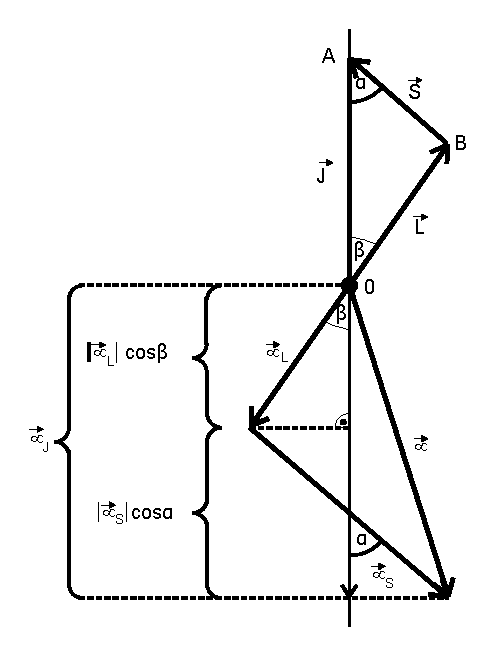
\includegraphics[width= 0.4 \linewidth]{pictures/Zeichnung1.pdf}
    \caption{Vektordiagramm der Drehimpulsvektoren einer Elektronenhülle und den daraus resultierenden magnetischen Momenten \cite{v606}.}
    \label{fig:Zeichnung1}
\end{figure}
Der Gesamtdrehimpuls $\vec{J}$ setzt sich aus drei Anteilen zusammen, welche auch schematisch in \autoref{fig:Zeichnung1} dargestellt sind.
Einmal der Bahndrehimpuls der Elektronenhülle, dem Eigendrehimpuls der Elektronen, auch Spin genannt, und der Kerndrehimpuls.
Letzterer kann hier vernachlässigt werden.
Es folgt also
\begin{equation}
    \vec{J} = \vec{L} + \vec{S},
\end{equation}
wobei $\vec{L}$ und $\vec{S}$ jeweils die Vektorsummen der Einzeldrehimpulse der Elektronen in der Hülle sind.
Quantenmechanisch lässt sich jetzt zeigen, dass
\begin{align}
    \vec{\mu_L} &= - \frac{\vec{\mu_B}}{\hbar} \vec{L} \quad \text{und} \\
    \vec{\mu_S} &= - \text{g}_S \frac{\vec{\mu_B}}{\hbar} \vec{S}
\end{align}
ist.
Dabei ist $\vec{\mu_B}$ das Bohrsche Magneton und $\text{g}_S$ das gyromagnetische Verhältnis des freien Elektrons.
Interessant sind oft die Beträge.
Mit
\begin{equation*}
    \left| \vec{J}\right| = \sqrt{J \left( J + 1 \right)} \cdot \hbar
\end{equation*}
folgt 
\begin{align}
    \left|\vec{\mu_L} \right| &= \mu_B \sqrt{L \left( L + 1 \right)} \\
    &\text{und} \nonumber \\
    \left|\vec{\mu_S} \right| &= \text{g}_S \mu_B \sqrt{S \left( S + 1 \right)}.
\end{align}
Durch einige geometrischen Beziehungen die sich aus \autoref{fig:Zeichnung1} entnehmen lassen und der Näherung von $\text{g}_S \approx 2$ folgt dann schließlich, dass
\begin{equation}
    \left|\vec{\mu}_{\mathrm{J}}\right| \approx \mu_{\mathrm{B}} \sqrt{\mathrm{J}(\mathrm{J}+1)} \frac{3 \mathrm{~J}(\mathrm{~J}+1)+\{\mathrm{S}(\mathrm{S}+1)-\mathrm{L}(\mathrm{L}+1)\}}{2 \mathrm{~J}(\mathrm{~J}+1)} .
\end{equation}
Dabei wird der Term
\begin{equation}
    g_{J}:=\frac{3 \mathrm{~J}(\mathrm{~J}+1)+\{\mathrm{S}(\mathrm{S}+1)-\mathrm{L}(\mathrm{L}+1)\}}{2 \mathrm{~J}(\mathrm{~J}+1)}
\end{equation}
der Landé-Faktor des betreffenden Atoms genannt. Damit gilt
\begin{equation}
    \left|\vec{\mu}_{\mathrm{J}}\right| \approx \mu_{\mathrm{B}} \mathrm{g}_{\mathrm{J}} \sqrt{\mathrm{J}(\mathrm{J}+1)}.
\end{equation}
Durch das quantenmechanische Phänomen der Richtungsquantelung gilt
\begin{equation}
    \mu_{J_z} = - \mu_B \text{g}_J m,
\end{equation}
wobei $m$ die Orientierungszahl ist.
Es lässt sich nun durch längere Rechnung zeigen, dass
\begin{equation}
    \chi=\frac{\mu_{0} \mu_{\mathrm{B}}^{2} \mathrm{~g}_{\mathrm{J}}^{2} \mathrm{NJ}(\mathrm{J}+1)}{3 \mathrm{kT}}
\end{equation}
ist \cite{v606}.
Dabei ist $N$ die Anzahl der Momente pro Volumeneinheit und $k$ die Boltzmann-Konstante.
Es lässt sich auch das Curiesche Gesetz des Paramagnetismus
\begin{equation}
    \chi \sim \frac{1}{T}
\end{equation}
erkennen.

Bekanntermaßen lässt sich Paramagnetismus sehr gut bei Verbindungen beobachten, die Ionen Seltener Erden enthalten.
Daraus lässt sich nach obigen Eigenschaften des Paramagnetismus folgern, dass die Elektronenhüllen dieser Verbindungen große Drehimpulse haben müssen.
Diese können nur durch die inneren Elektronen erzeugt werden, genauer gesagt durch die Elektronen in der 4f-Schale.
Die Anordnung der Elektronen in dieser Schale und der daraus resultierende Gesamtdrehimpuls $\vec{J}$ werden durch die sogenannten Hundschen Regeln beschrieben.
Diese lauten:
\begin{enumerate}
    \item Die Spins $\vec{s_i}$ kombinieren zum Gesamtspin $\vec{S} = \sum \vec{s_i}$ , die nach dem Pauli-Prinzip gebildet werden können
    \item Der maximale Drehimpuls $\vec{L} = \sum \vec{l_i}$ entsteht so, dass die Bahndrehimpulse $\vec{l_i}$ mit dem Pauli-Prinzip und der ersten Regel verträglich sind.
    \item Der Gesamtdrehimpuls ist $\vec{J} = \vec{L} - \vec{S}$, falls die Schale weniger als zu Hälfte gefüllt ist und $\vec{J} = \vec{L} + \vec{S}$, wenn sie mehr als zur Hälfte gefüllt ist.
\end{enumerate}

Diese Regeln basieren darauf, dass die Hüllenelektronen sich untereinander elektrostatisch abstoßen.


\subsection{Vorgehen zur Bestimmung der Suszeptibilität}
\begin{wrapfigure}{r}{0.4\linewidth}
    \center
    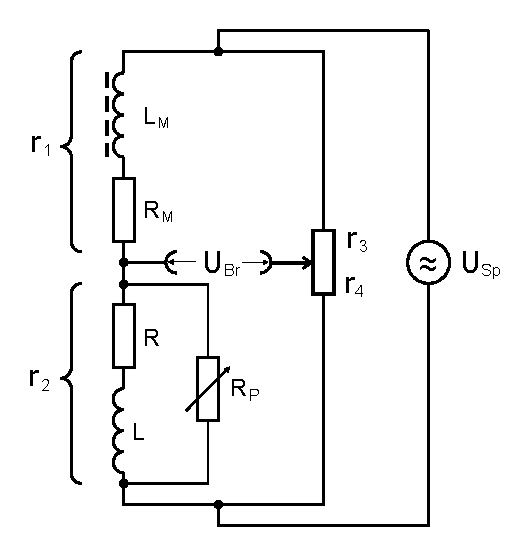
\includegraphics[width=\linewidth]{pictures/Zeichnung2.pdf}
    \caption{Suszeptibilitätsmessung mittels einer Brückenschaltung \cite{v606}.}
    \label{fig:Zeichnung2}
\end{wrapfigure}
Um die Suszeptibilität $\chi$ experimentell zu bestimmen, wird eine Brückenschaltung wie in \autoref{fig:Zeichnung2} verwendet.
Die Induktivität einer Spule ist durch
\begin{equation}
    L_\text{ges} = \mu \mu_0 \frac{n^2}{I} F
\end{equation}
gegeben, welche sich aber aufgrund der technischen Realisierbarkeit zu
\begin{equation}
    L_\text{ges} ' = \mu_0 \frac{n^2}{I} F + \chi \mu_0 \mu_0 \frac{n^2}{I} Q
\end{equation}
abändert. Dabei ist $Q$ der Querschnitt der Probe und $F$ der Spulenquerschnitt.
Es werden zwei Spulen möglichst gleicher Induktivität $L$ benutzt, da die Induktionsdifferenz $\increment L$ für die Suszeptibilitätsmessung entscheidend ist.
Nach langer Rechnung lässt sich für den hohe Frequenzen zeigen, dass
\begin{equation}
    \omega \rightarrow \inf: \chi = 2 \cdot \frac{\increment R}{R_3} \frac{F}{Q}
\end{equation}
gilt.
$R_3$ ist dabei der Widerstand am Potentiometer in \autoref{fig:Zeichnung2} und $\increment$ die Differenz am Potentiometer.
\section{Durchführung} \label{sec:Durchführung}



\subsection{Technische Daten} \label{sec:Daten}
Im Folgenden werden zunächst die technischen Daten der einzelnen Komponenten etc aufgelistet:
\begin{align*}
    \textbf{Dopplerphantomflussigkeit:} && \rho &= 1,15  \unit\gram / \unit{\cubic\centi\meter} & \text{Dichte} \\
    && c_L &= 1800 \unit\meter / \unit\second & \text{Schallgeschwindigkeit} \\
    && \nu &= 12 \unit{\milli\pascal\second} & \text{Viskosität} \\
    \\
    \textbf{Dopplerprisma:} && c_P &= 2700 \unit\meter / \unit\second & \text{Schallgeschwindigkeit} \\
    && l &= 30,7 \unit{\milli\meter} & \text{Länge der Vorlaufstrecke} \\
    \\
    \textbf{Strömungsrohre:} && \text{Innendurchmesser} && \text{Außendurchmesser} \\
    && 7 \unit{\milli\meter} && 10 \unit{\milli\meter} \\
    && 10 \unit{\milli\meter} && 15 \unit{\milli\meter} \\
    && 16 \unit{\milli\meter} && 20 \unit{\milli\meter} \\
\end{align*}

% \subsection{Vorbereitungsaufgabe}
% Die Dopplerwinkel berechnen sich nach der Formel
% \begin{equation}
%     \alpha = 90° - \text{arcsin}\left(\text{sin} \theta \frac{c_L}{c_P}\right).
% \end{equation}
% Daraus folgt für
% \begin{align*}
%     \theta_1 &= 15° &\implies&& \alpha_1 &= 80,06°, \\
%     \theta_2 &= 30° &\implies&& \alpha_2 &= 70,53°, \\
%     \theta_3 &= 60° &\implies&& \alpha_3 &= 54,74°. \\
% \end{align*}

\subsection{Aufbau}
Der Aufbau besteht aus einem Flüssigkeitskreislauf, an dem eine Zentrifugalpumpe angeschlossen ist.
Die Pumpe erzeugt die Strömung innerhalb der Strömungsrohre. Die Geschwindigkeit des Durchflusses kann stufenlos
durch die Pumpleistung geregelt werden. Innerhalb der Rohre befindet sich die Dopplerphantomflüssigkeit.
\begin{wrapfigure}{r}{0.3\linewidth}
    \center
    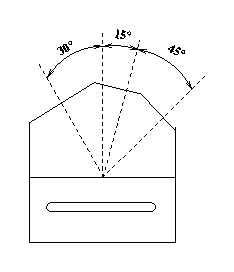
\includegraphics[width=\linewidth]{pictures/Skizze2.pdf}
    \caption{Das Dopplerprisma. \cite{us3}}
    \label{fig:Skizze2}
\end{wrapfigure}
In diesem Kreislauf sind verschiedene Rohrstücke mit verschiedenen Durchmessern eingebaut, siehe dafür \hyperref[sec:Daten]{Kapitel \ref{sec:Daten}}.
Auf diese Rohrstücke wird jeweils ein Dopplerprisma aus Acryl montiert.
Wie in der \hyperref[fig:Skizze2]{Abbildung \ref{fig:Skizze2}} zu erkennen, lassen sich darauf drei Winkel einstellen.
Die Kontaktflächen werden vorher mit einem speziellen Gel bedeckt.
Dass dient der besseren Übertragung der Ultraschallwellen.
Es wird eine Schallfrequenz $\nu_0$ eingestellt.
Die Sonde ist indirekt mit dem Computer verbunden. Dort lässt sich direkt über das Programm \enquote{FlowView} die Messwerte ablesen.
\subsection{Durchführung}
Zunächst wird der Laptop angeschaltet, um das Programm \enquote{FlowView} zu verwenden.
Dann wird die maximale Leistung des Motors aufgeschrieben, die in diesem Falle bei 9000 Umdrehungen lag.
Der Prisma und die Sonde wird mit dem Gel benetzt.
Schließlich wird das Gerät der Sonde eingeschaltet und für die erste Messung wird das \enquote{SAMPLE VOLUME} auf HIGH gestellt.
Es wird dann für verschiedene Flussgeschwindigkeiten bei den drei Winkeln am Prisma eine Messung durchgeführt
und bei Flowview ein Screenshot erstellt, woraus sich dann die Messwerte für die Auswertung extrahieren lassen.
Dies wird für verschiedene Anteile der Maximalleistung durchgeführt.

Bei der zweiten Messreihe wird das das SAMPLE VOLUME auf SMALL gestellt.
Die Messtiefe wird über den Regler Depth geregelt.
Diese Messung wird jeweils für 75 \% der Messtiefe und 45 \% durchgeführt.
%\section{Fehlerrechnung}
\label{sec:Fehlerrechnung}

Im Folgenden wird die allgemeine Fehlerrechnung und alle wichtigen Größen der entsprechenden Rechnung erklärt.
Die wichtigsten Werte dabei sind der 
\begin{align}
    \text{Mittelwert} \quad & \bar{x}  = \frac{1}{N} \sum_{i=0}^{n} x_i \quad \text{und die} \label{eq:mittelwert} \\
    \text{Standartabweichung} \quad & \sigma  = \sqrt{\frac{1}{N - 1 } \sum_{i=0}^{N} (x_i -  \bar{x})^2} \, . \label{eq:standartabweichung}
\end{align}

Dabei entspricht $N$ der Anzahl an Werten und $x_i$ ist jeweils ein mit einem Fehler gemessener Wert.
Es ergibt sich ebenfalls die statistische Messunsicherheit
\begin{equation}
    \increment \bar{x} = \frac{\sigma}{\sqrt{N}} = 
    \sqrt{\frac{1}{N(N - 1)} \sum_{i=0}^{N} (x_i -  \bar{x})^2} \, . \label{eq:messunsicherheit}
\end{equation} 

Entstehen mehrere Unbekannte in einer Messung, folgen daraus auch mehrere Messunischerheiten,
die in dem weiteren Verlauf der Rechnung berücksichtigt werden müssen.
Es gilt die \textit{Gaußsche Fehlerfortplanzung}
\begin{equation}
    \increment f(y_1 ,y_2 ,...,y_N ) = \sqrt{\left(\frac{\dif{f}}{\dif{y_{1}}} \increment y_{1}\right)^2
    + \left(\frac{\dif{f}}{\dif{y_{2}}} \increment y_{2}\right)^2 + ... + 
    \left(\frac{\dif{f}}{\dif{y_{N}}} \increment y_{N}\right)^2
    } \, . \label{eq:fehlerfortplanzung}
\end{equation}
\section{Auswertung}
\label{sec:Auswertung}


Im folgenden werden die Theoriewerte aus \autoref{tab:literatur}, die der Literatur entnommen wurden, verwendet \cite{x_ray_database}.
Die zugehörigen Winkel jeweiliger Materialien wurden dann nach \autoref{eq:tbd} berechnet.
Es folgt 
\begin{equation*}
  \theta = \arcsin \left( \frac{h c}{2 d E} \right)
\end{equation*}
Dabei wurde $n = 1$ gesetzt und $\lambda$ durch die bekannte Gleichung 
\begin{equation*}
  \lambda = \frac{h \cdot c}{E}
\end{equation*}
berechnet.
Weiterhin werden für die Theoriewerte der Kupferlinien
\begin{align*}
  E_{\mathrm{K}, \mathrm{abs}} &=8,987 \mathrm{keV} \, \\
  E_{\mathrm{K}, \alpha}^{\mathrm{lit}} &=8,048 \mathrm{keV} 
\end{align*}
und
\begin{equation*}
  E_{\mathrm{K}, \beta}^{\mathrm{lit}} =8,906 \mathrm{keV} \, .
\end{equation*}
angenommen \cite{x_ray_database}.
Daraus resultieren dann auch durch \autoref{eq:sigma} die $\sigma_i$'s
\begin{align*}
  \sigma_{1} &=3,29 \, ,\\
  \sigma_{2} &=12,38 \\ 
  \intertext{und}
  \sigma_{3} &=21,68 \, .
\end{align*}
 
\begin{table}
  \centering
  \caption{Theoriewerte für die Messwerte \cite{x_ray_database}.}
  \label{tab:literatur}
  \begin{tabular}{ccccc} 
    \hline Element & $Z$ & $\sigma_{\mathrm{K, Lit}}$& $E_{\mathrm{K, Lit}}$ in keV & $\theta_{\mathrm{K, Lit}}$ in \\
    \hline $\mathrm{Zn}$ & 30 & 3,57 & 9,65 & 18,60  \\
    $\mathrm{Ga}$ & 31 & 3,60 & 10,38 & 17,25  \\
    $\mathrm{Ge}$ & 32 & 3,66 & 11,11 & 16,08  \\
    $\mathrm{Br}$ & 35 & 3,84 & 13,48 & 13,20  \\
    $\mathrm{Rb}$ & 37 & 3,94 & 15,2 & 11,68   \\
    $\mathrm{Sr}$ & 38 & 3,98 & 16,12 & 11,01  \\
    $\mathrm{Zr}$ & 40 & 4,09 & 18,0 & 9,85    \\
    \hline
  \end{tabular}
\end{table}

\subsection{Überprüfung der Bragg - Bedingung}
Zunächst soll die Bragg-Bedingung nachgewiesen werden.
Die Messwerte sind in \autoref{fig:bragg} aufgetragen.
Der Sollwinkel liegt bei $28°$.
Mittels Python wurde das Maximum bei $28°$ gefunden.

\begin{figure}
  \centering
  \caption{Messwerte zur Untersuchung der Bragg-Bedingung}
  \label{fig:bragg}
  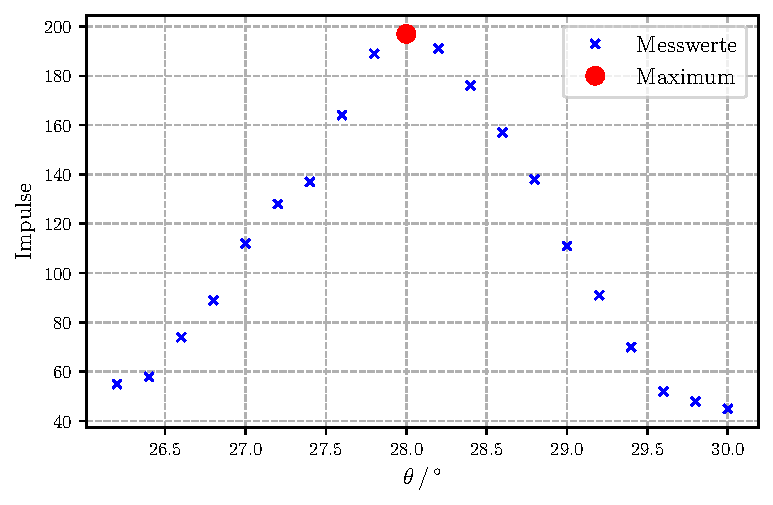
\includegraphics[width=0.5 \linewidth]{build/bragg.pdf}
\end{figure}

\subsection{Emissionsspektrum von Kupfer}
Im folgenden wird das Emissionsspektrum von Kupfer untersucht.
Aufgetragen sind die Messdaten, die über einen USB-Stick beim Versuch gespeichert und ausgelesen wurden, in \autoref{fig:kupfer1}.
Das Maximum der Bremsstrahlung wurde ebenfalls per Python bei $\qty{11.8}{°}$ ermittelt.  
Um die charakteristische Strahlung genauer zu untersuchen werden nur Messwerte zwischen tbd und tbd in \autoref{fig:kupfer2} abgebildet.
Aus den Peaks lassen sich dann die Energien mit \autoref{eq:tbd} zu
\begin{align*}
  E_{\text{K}_\alpha} = \qty{8.077}{keV} &&\text{und}&& E_{\text{K}_\beta} = \qty{8.914}{keV}
\end{align*}
berechnet.
Die Halbwertsbreiten liefern die Energiedifferenzen
\begin{align*}
  \increment E_{\text{K}_\alpha} = \qty{154.5}{keV} &&\text{und}&& \increment E_{\text{K}_\beta} = \qty{195.8}{keV} \, .
\end{align*}
Für das Auflösungsvermögen gilt die Gleichung
\begin{equation*}
  A = \frac{E}{\increment E} \, ,
\end{equation*}
woraus die Werte
\begin{align*}
  A_{\text{K}_\alpha} = 41,24 && \text{und} && A_{\text{K}_\beta} = 57,69
\end{align*}
bestimmt werden.
Schließlich werden noch die Abschirmkonstanten mit \autoref{tbd}, \autoref{tbd} und \autoref{tbd} bestimmt.
Hier wird für das Errechnen von $\sigma_2$ und $\sigma_3$ der theoretische Wert von $\sigma_1$ herangezogen, da sonst keine Bestimmung der anderen Möglich wäre. 
Es folgt
\begin{align*}
  \sigma_{1} &= 3,29 \, ,\\
  \sigma_{2} &= 12,62 \\ 
  \intertext{und}
  \sigma_{3} &= 21.93 \, .
\end{align*}

\begin{figure}
  \centering
  \caption{Messreihe zur Untersuchung des Emissionsspektrums von Kupfer.}
  \label{fig:kupfer1}
  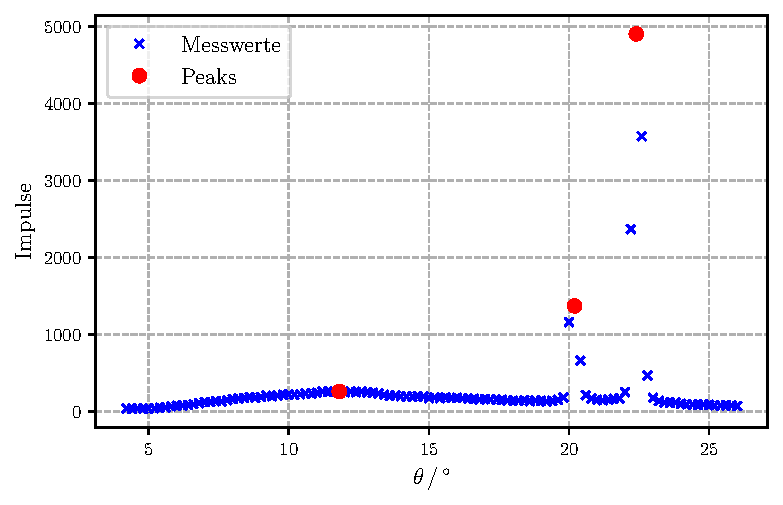
\includegraphics[width=0.5 \linewidth]{build/kupfer1.pdf}
\end{figure}

\begin{figure}
  \centering
  \caption{ Messreihe zur genaueren Untersuchung des Emissionsspektrums von Kupfer.}
  \label{fig:kupfer2}
  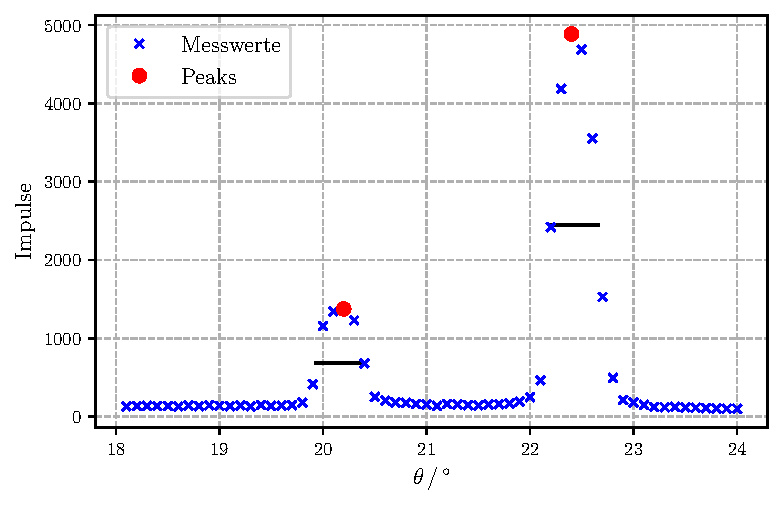
\includegraphics[width=0.5 \linewidth]{build/kupfer2.pdf}
\end{figure}

\subsection{Analyse der Absorptionsspektren}

Abschließend sollen die Absorptionsspektren verschiedenster Materialien ermittelt werden.
Hierfür wird die Zählrate $N$ der gemessenen Impulse gegen den Winkel $\theta$ aufgetragen.
Die Absorptionskante wird in den folgenden Plots eingezeichnet.
Zusätzlich wird eine vertikale Linie durch die Mitte dieser Kante gelegt.
Die Mitte ist durch die Gleichung
\begin{equation*}
  I_K = \frac{I_K^\text{min} + I_K^\text{max}}{2}
\end{equation*}
festgelegt. Dabei beschreiben $I_K^\text{min}$ und $I_K^\text{max}$ das Intensitätsminimum /- maximum der Absorptionskante.
Daraus lässt sich dann der Winkel $\theta$ bestimmen, woraus Schließlich die Energie sowie die Abschirmkonstante bestimmt werden kann.

\subsubsection{Zink}
% \begin{figure}
%   \centering
%   \caption{Absorptionsspektrum von Zink.}
%   \label{fig:zink}
%   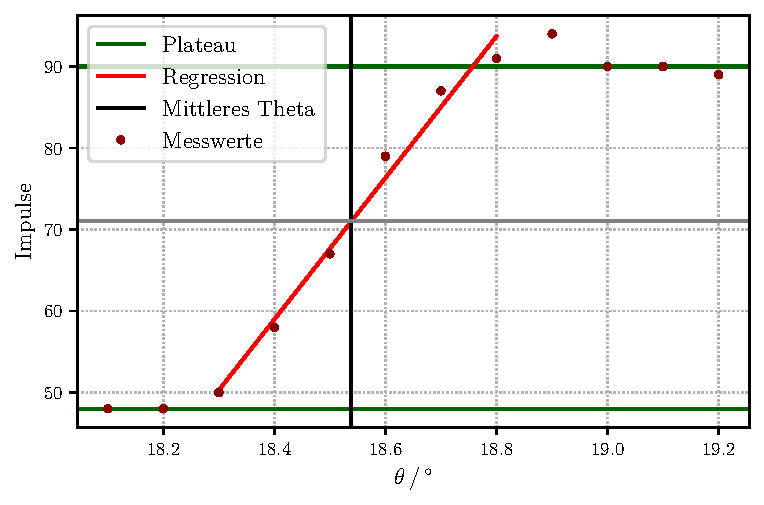
\includegraphics[width=0.5 \linewidth]{build/zink.pdf}
% \end{figure}

\subsubsection{Gallium}
% \begin{figure}
%   \centering
%   \caption{Absorbtionsspektrum von Gallium.}
%   \label{fig:gallium}
%   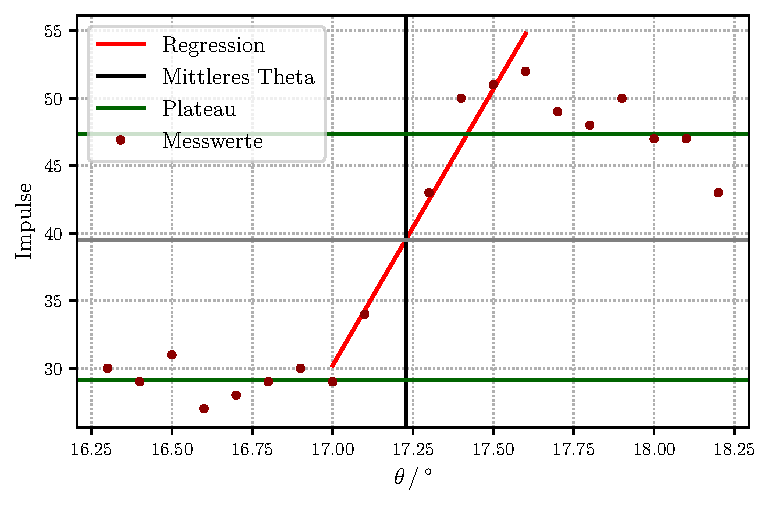
\includegraphics[width=0.5 \linewidth]{build/gallium.pdf}
% \end{figure}

\subsubsection{Brom}
% \begin{figure}
%   \centering
%   \caption{Absorbtionsspektrum von Brom.}
%   \label{fig:brom}
%   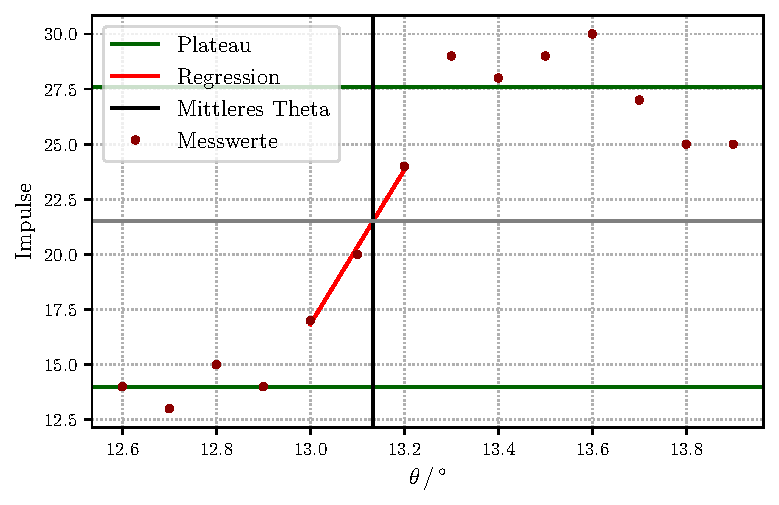
\includegraphics[width=0.5 \linewidth]{build/brom.pdf}
% \end{figure}

\subsubsection{Rubidium}
% \begin{figure}
%   \centering
%   \caption{Absorbtionsspektrum von Rubidium.}
%   \label{fig:rubidium}
%   \includegraphics[width=0.5 \linewidth]{build/rubidium.pdf}
% \end{figure}

\subsubsection{Strontium}
% \begin{figure}
%   \centering
%   \caption{Absorbtionsspektrum von Strontium.}
%   \label{fig:strontium}
%   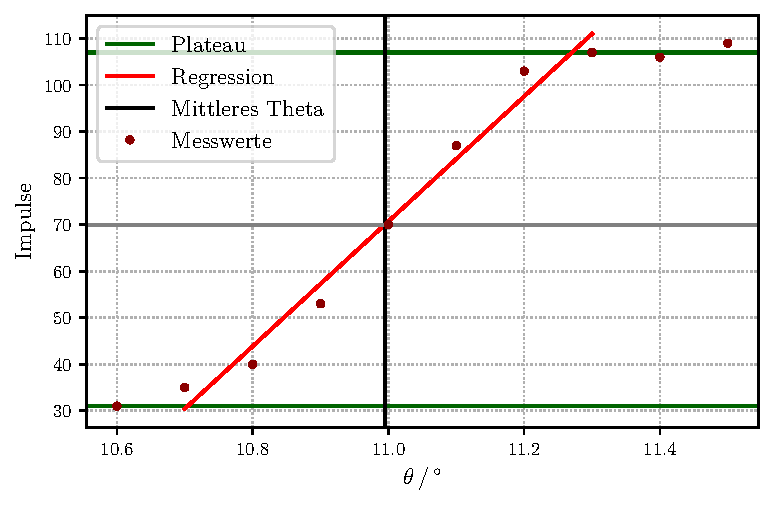
\includegraphics[width=0.5 \linewidth]{build/strontium.pdf}
% \end{figure}

\subsubsection{Zirkonium}
% \begin{figure}
%   \centering
%   \caption{Absorbtionsspektrum von Zirkonium.}
%   \label{fig:zirkonium}
%   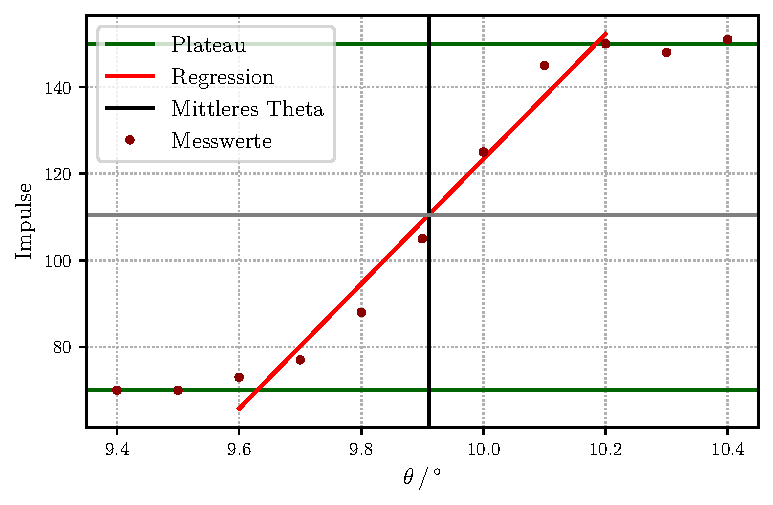
\includegraphics[width=0.5 \linewidth]{build/zirkonium.pdf}
% \end{figure}

\subsection{Moseley's Gesetz}
Nun wird mit den gewonnenen Energien das Moseley'sche Gesetz verifiziert werden.
Hierfür wird der Ansatz
\begin{equation*}
  f(Z) = m \cdot Z + b
\end{equation*}
gewählt. Dabei werden die Wurzeln der ermittelten Energien gegen die zugehörigen $Z$'s aufgetragen.
Die Regression ist dargestellt in \autoref{fig:moseley}.
Aus der linearen Regression mittels Python ergeben sich die Parameter
\begin{align*}
  m = \qty{1}{\eV}^{-\frac{1}{2}} && \text{und} && b  = \qty{1}{\eV}^{-\frac{1}{2}} \, .
\end{align*}
Daraus lässt sich nun die experimentell ermittelte Rydberg-Energie zu
\begin{equation*}
  E_\text{Ryd} = \frac{1}{m^2} = tbd
\end{equation*}
berechnen.

% \begin{figure}
%   \centering
%   \caption{Regressionsgerade zur Verifizierung des Moseley'schen Gesetzes.}
%   \label{fig:moseley}
%   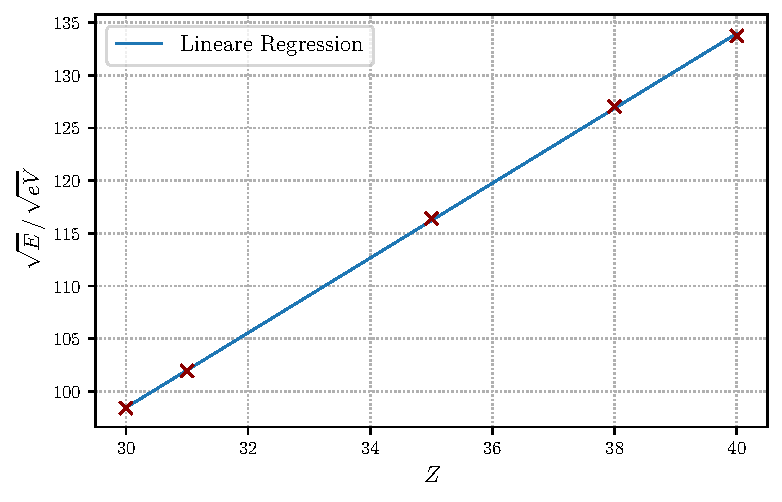
\includegraphics[width=0.5 \linewidth]{build/moseley.pdf}
% \end{figure}
\section{Diskussion}
\label{sec:Diskussion}

\subsection{Ausmessung des Acrylblocks mittels A-Scan}

Da während der Messung der Störstellen eins und zwei keine weitere Sonden-Frequenz gemacht wurde, 
konnte keine axiale Auflösung zweier benachbarter Störstellen im Acrylblock bestimmt werden.
Des Weiteren soll erwähnt sein, dass die Störstelle 10 beim A- und B-Scan von der Störstelle 11 verdeckt wurde und daher keine Aufnahme von unten möglich war, 
von oben jedoch schon.

Im Vergleich der experimentell bestimmten Durchmesser der Störstellen in \autoref{tab:vgl} ergeben sich die in \autoref{tab:abw} dargestellten Abweichungen.
\begin{table}[H]
    \centering
    \caption{Die berechneten Durchmesser im Vergleich mit den gemessenen.}
    \label{tab:vgl}
    \begin{tabular}{c c c c}
        \toprule
        Stelle &
        $d_\text{Loch} \mathbin{/} \unit{\milli\meter}$ (A-Scan) &
        $d_\text{Loch} \mathbin{/} \unit{\milli\meter}$ (B-Scan) & 
        $d_\text{Loch} \mathbin{/} \unit{\milli\meter}$ \\
        \midrule
                3 &             4,32 &             5,28 &           5,80 \\
                4 &             3,37 &             4,87 &           4,70 \\
                5 &             3,23 &             2,55 &           3,60 \\
                6 &             3,37 &             2,82 &           2,86 \\
                7 &             1,86 &             2,55 &           2,86 \\
                8 &             4,87 &             2,82 &           2,86 \\
                9 &             1,05 &             2,68 &           2,86 \\
                10 &                  &                  &           2,86 \\
                11 &             8,83 &             9,37 &           9,00 \\
        \bottomrule
    \end{tabular}
\end{table}

\begin{table}
    \centering
    \caption{Die relativen Abweichungen der bestimmten Durchmesser.}
    \label{tab:abw}
    \begin{tabular}{c c c}
        \toprule
        Stelle &
        $\increment d_\text{Loch} \mathbin{/} \%$ (A-Scan) &
        $\increment d_\text{Loch} \mathbin{/} \%$ (B-Scan) \\
        \midrule
         3 &  25,52 &                   8,97 \\
         4 &  28,30 &                   3,62 \\
         5 &  10,28 &                  29,17 \\
         6 &  17,83 &                   1,40 \\
         7 &  34,97 &                  10,84 \\
         8 &  70,28 &                   1,40 \\
         9 &  63,29 &                   6,29 \\
         10 &       &                        \\
         11 &  1,89 &                   4,11 \\
        \bottomrule
    \end{tabular} 
\end{table}

Neben der allgemeinen Messung mit der Sonde, fiel das Ablesen der Laufzeiten in \autoref{sec:a-scan} und \autoref{sec:b-scan} schwer,
da der Cursor im Messprogramm verwendet wurde.  
Weitere Fehlerquellen für die sporadischen Abweichungen finden sich in der Herausforderung, klare Aufnahmen beim B-Scan zu machen, 
während die Sonde über den Acrylblock geführt wird.


\subsection{Bestimmung der Lage und Größe der Tumore im Brustmodell}

Im Vergleich zum zweiten Tumor ist bei der Aufnahme des ersten Tumor ein klarer Peak zu erkennen, 
der auf eine härteres Hindernis und daher auf den festen Tumor schließen lässt.
Der zweite hingegen lässt einen weiteren Peak nach dem ersten erkenne, was als ein Hohlraum gedeutet werden kann.
Der Tumor auf der rechten Seite kann daher als Zyste identifiziert werden.
Ein B-Scan, auf dem ein klarer Unterschied der beiden Geschwüre erkenntlich ist, konnte nicht gemacht werden.

\newpage
\printbibliography{}
\nocite{matplotlib}
\nocite{numpy}
\nocite{scipy}
\nocite{uncertainties}
\nocite{reback2020pandas}

\newpage
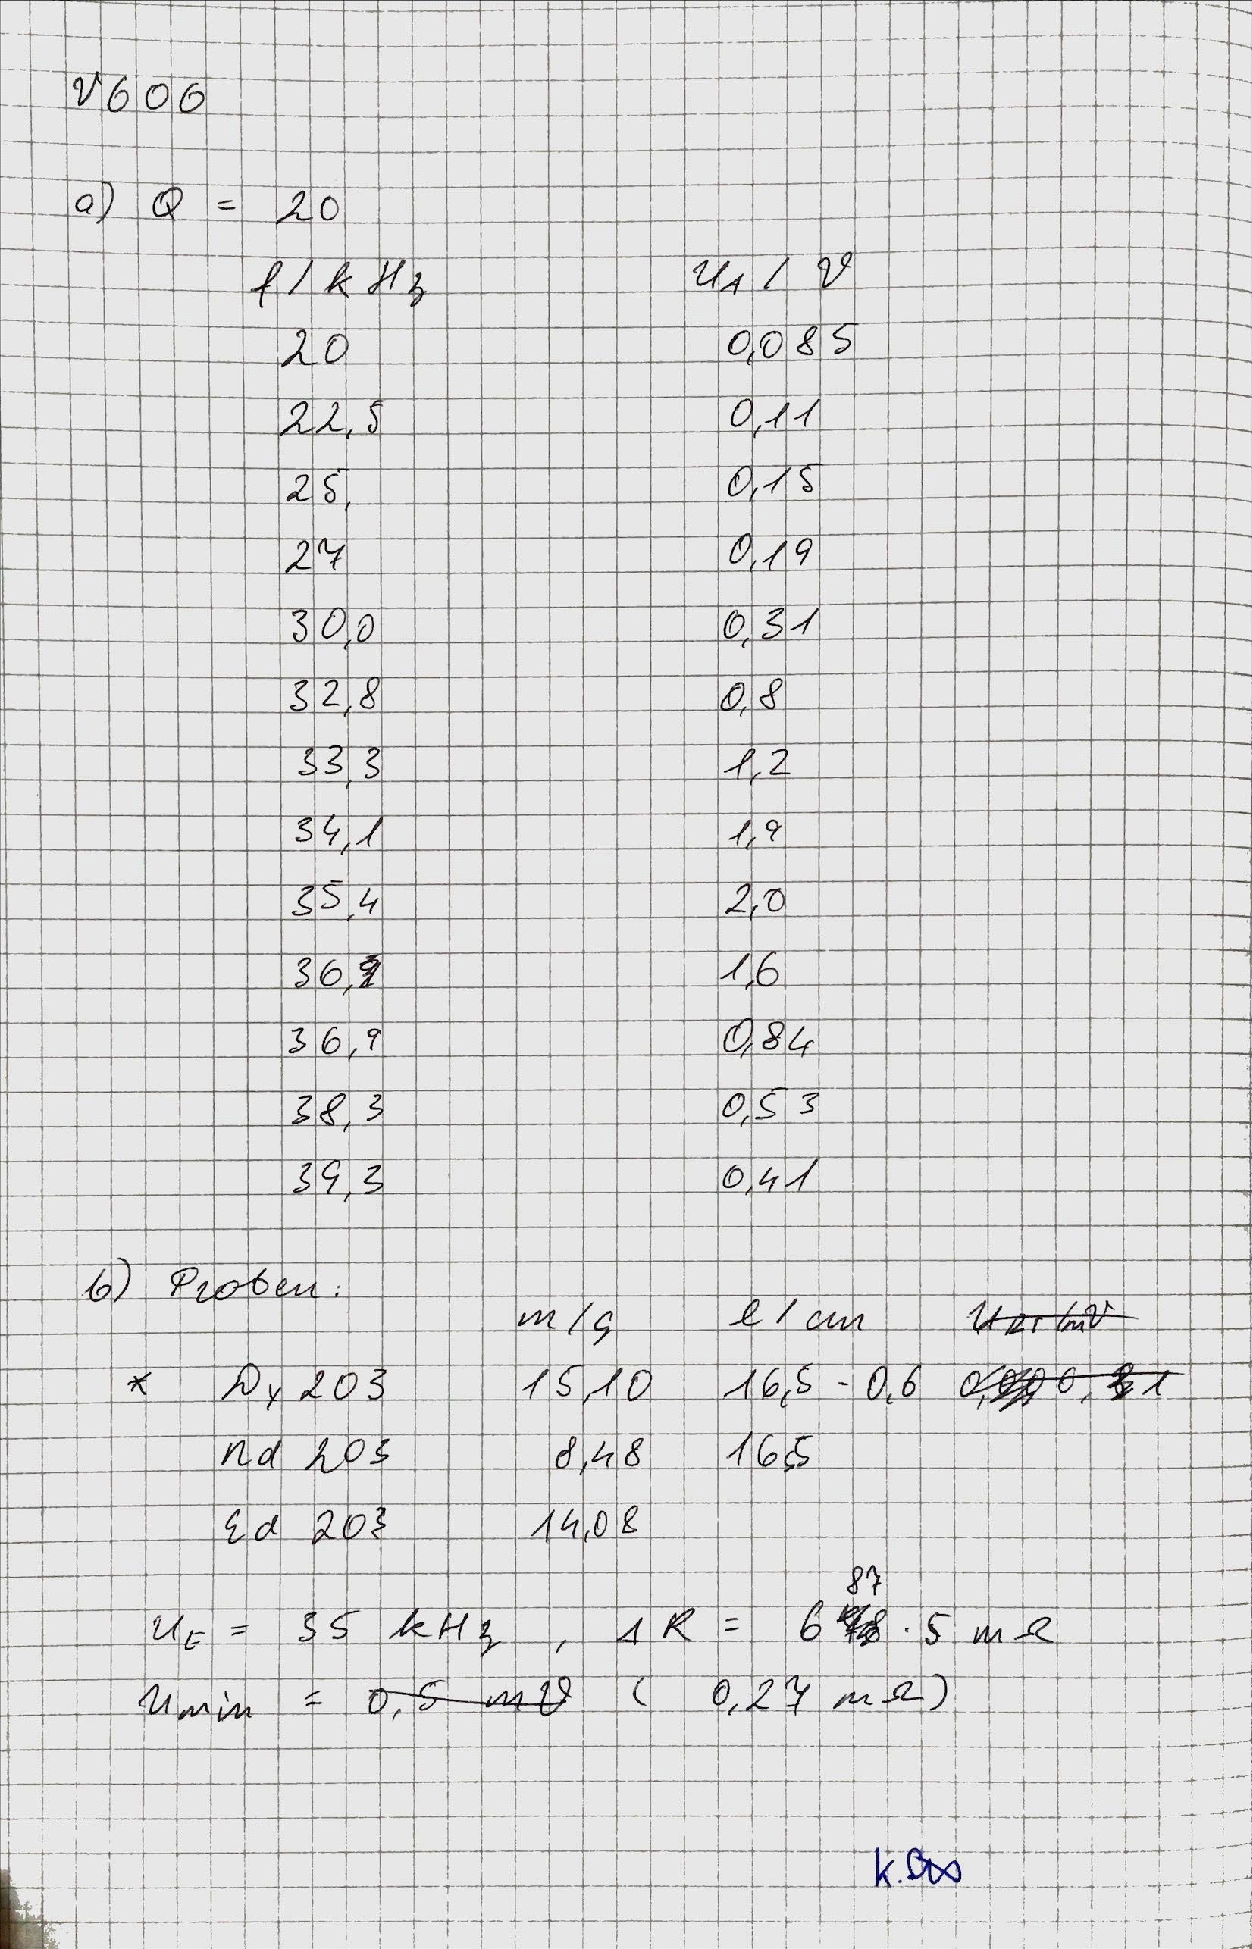
\includepdf[pages=-]{tables/messdaten.pdf}

\end{document}